Rather than looking at an explicit representation of lines in the plane, we can gain much more insight from looking at a parametric representation. To simplify our analysis, we will choose our time parameter such that v collisions occur every $\Delta t = 1$ and h collisions occur every $\Delta t = \frac{1}{m}$. The equation for a line $y(x) = m \, x + b$ is equivalent to the following parametric system

\begin{align}\label{eq:parametric-line}
	x(t) = t + x_0\\
	y(t) = m \, t
\end{align}

Now our v and h collisions in the 2-dimensional plane can be projected onto the 1-dimensional parametric representation.

\begin{figure}[H]
  \begin{center}
    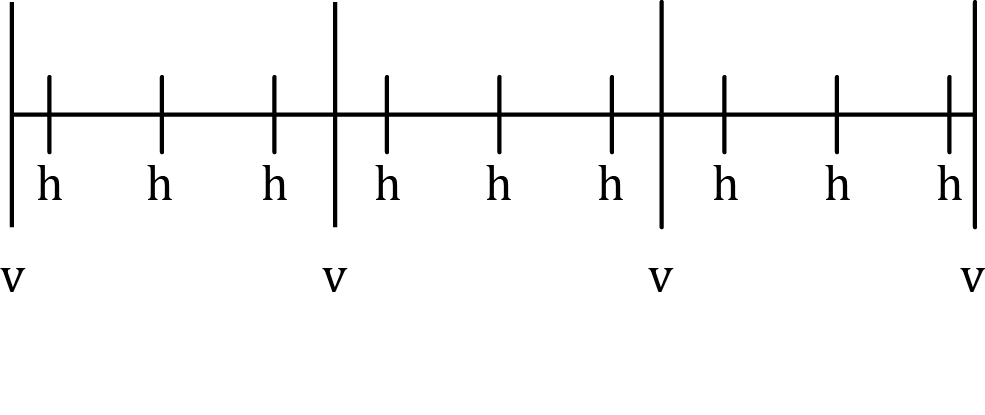
\includegraphics[keepaspectratio, width=4in]{1d_mapping_2.png}
  \end{center}
  \vspace{-.2in} % corrects bad spacing
  \caption{\label{fig:1d-projection} Projecting onto the parametric representation.}
\end{figure}

We will occasionally have to deal with some boundary conditions, and we will introduce some intermediate sequences which we will label as `augmented' and mark with a tilde. The boundary treatments are fairly pedantic and can be ignored if the reader is just interested in getting a general understanding of our solutions.

All of our theorems in this section will rely on the lengths of various patterns in the original collision sequence. We will start off by looking at the lengths of subsequences of v collisions in the collision sequence. To make this accounting simpler, we need to define an augmented collision sequence.

\begin{definition}
	\textbf{augmented collision sequence ($\tilde{\alpha}$)} which consists of the original collision sequence with one h collision added to both ends of the sequence.
\end{definition}

Now we can count lengths of v collision substrings

\begin{definition}
	\textbf{Augmented $\beta_i$:} number of v collisions between i\textsuperscript{th} and (i+1)\textsuperscript{th} h collisions in the augmented collision sequence
\end{definition}

\textbf{Still working on this part, not sure how best to deal with the boundary conditions...}

The first and last numbers in the $\beta$ sequence were artificially created by augmenting our original collision sequence. These two numbers only give us a lower bound on the number of v collisions between h collisions, so we can safely discard them if 

\begin{definition}
	\begin{align*}
		\beta_{min} \coloneqq \max_i \beta_i\\
		\beta_{max} \coloneqq \min_i \beta_i
	\end{align*}
\end{definition}

The $\beta$ sequence is much simpler to think of geometrically in terms of our parametric representation shown in Figure \ref{fig:1d-projection}. $\beta_i$ represents the number of v collision tick marks in between each h collision tick mark.

\begin{figure}[H]
  \begin{center}
    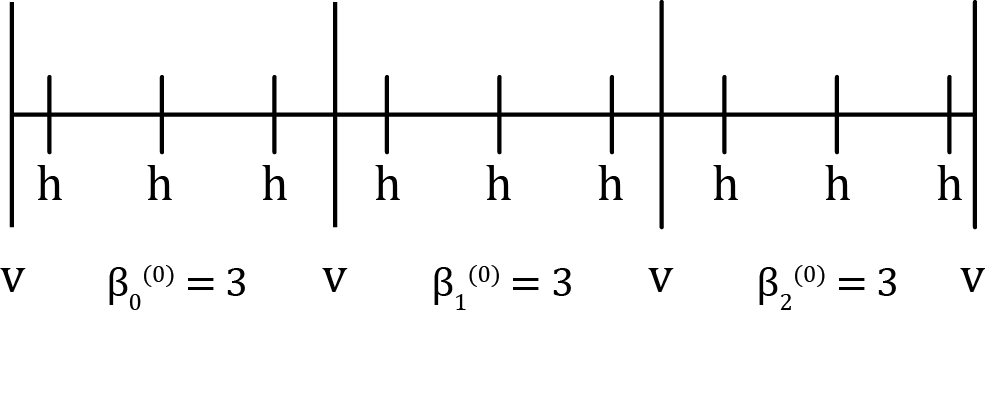
\includegraphics[keepaspectratio, width=4in]{1d_mapping_3.png}
  \end{center}
  \vspace{-.2in} % corrects bad spacing
  \caption{\label{fig:beta-sequence} The $\beta$ sequence.}
\end{figure}

\begin{lemma}
	\[
		\beta_{min} > 0
	\]
\end{lemma}

\begin{proof}
	TODO
\end{proof}

\begin{theorem}
	For every valid collision sequence, the following must be true
	
	\[
		\beta_{max} - \beta_{min} \le 1
	\]
\end{theorem}

\begin{proof}

From Equation \ref{eq:parametric-line}, v collisions occur every $\Delta t = 1$ and h collisions occur every $\Delta t = \frac{1}{m}$. Thus, the following must be true

\[
	\beta_i \in \paren{\floor{\frac{1}{m}}, \ceil{\frac{1}{m}}}
\]

For an $m$ to exist that satisfies the above constraints, all numbers in the $\beta$ sequence can only differ by 1.

\end{proof}

\begin{definition}
	\textbf{Augmented $C^{(0)}_i$:} 1 more than the number of occurrences of $\beta_{max}$ between i\textsuperscript{th} and (i+1)\textsuperscript{th} occurrence of $\beta_{min}$ in the $\beta$ sequence.
\end{definition}

\begin{theorem}
	Define 
	\begin{align*}
			\delta_i \coloneqq \begin{cases}
				x_0 \qquad &\text{if} \quad i = 0\\
				i (\ceil{\frac{1}{m}} - \frac{1}{m}) \qquad &\text{otherwise}
			\end{cases}
	\end{align*}

	Then the following is true for all valid collision sequences

	\begin{align*}
		\beta_i = \floor{\delta_i} + \beta_{max} - \floor{\delta_{i+1}}
	\end{align*}
\end{theorem}

\begin{proof}
	TODO...
\end{proof}